%%%%%%%%%%%%%%%%%%%%%%%%%%%%%%%%%%%%%%%%%%%%%%%%%%%%%%%%%%%
% | - Active Learning Machine Learning Results
% %%%%%%%%%%%%%%%%%%%%%%%%%%%%%%%%%%%%%%%%%%%%%%%%%%%%%%%%%
% TODO Change guiding lines of performance plot because 7/10 systems isn't the best metric anymore
%
% __|
%%%%%%%%%%%%%%%%%%%%%%%%%%%%%%%%%%%%%%%%%%%%%%%%%%%%%%%%%%%



% %%%%%%%%%%%%%%%%%%%%%%%%%%%%%%%%%%%%%%%%%%%%%%%%%%%%%%%%%
% | - Intro To Section
% Intro/transition paragraph
% __|
% %%%%%%%%%%%%%%%%%%%%%%%%%%%%%%%%%%%%%%%%%%%%%%%%%%%%%%%%%
% | - PARAGRAPH BODY
%
The AL algorithm is now applied to the discovery of stable and unique polymorphs of \IrOtwo and \IrOthree.
%
Since the algorithm is applied to each stoichiometry individually,
we will only illustrate the results for \IrOthree,
a comparatively unstudied oxide system.
%
% TODO I don't talk about IrO2 enough
We will briefly touch on the results for \IrOtwo at the end and refer the reader to the Supporting Information for further details.
% __|
%%%%%%%%%%%%%%%%%%%%%%%%%%%%%%%%%%%%%%%%%%%%%%%%%%%%%%%%%%%


% %%%%%%%%%%%%%%%%%%%%%%%%%%%%%%%%%%%%%%%%%%%%%%%%%%%%%%%%%
% | - AL Results for IrO3
% * Introduce the convergence plots
% * The GP becomes more accurate as more DFT is acquired
% * The GP can start to recognize the low energy systems after minimal DFT
%
% We need to call them something else than "convergence plots" (bad name)
% __|
% %%%%%%%%%%%%%%%%%%%%%%%%%%%%%%%%%%%%%%%%%%%%%%%%%%%%%%%%%
% | - PARAGRAPH BODY
%
Figure~\ref{fig:iro3_al}a, shows a sequence of snapshots of the AL algorithm at different generations for \IrOthree.
%
Each subplot reports the predicted (hollow grey) and DFT-derived (solid red) formation enthalpies (\DHf) for each structure, sorted by stability.
%
As the algorithm acquires DFT data, the GP model's accuracy increases,
as evidenced by the decreasing uncertainties when comparing the initial and latter generations (\ref{fig:iro3_al}a.i-v).
%
At the top of each subplot of Figure~\ref{fig:iro3_al}a the x-axis positioning of the ten most stable polymorphs is tracked.
%
Initially, these ten structures are randomly distributed across the entire candidate space due to the insufficiently trained GP model.
%
But, after only three generations (Figure~\ref{fig:iro3_al}a.ii) the GP model is sufficiently accurate to predict the most stable polymorphs as being low energy.
%
By the fifth generation (\num{30} DFT relaxations) \num{4/10} of the most stable polymorphs have been acquired,
including the globally stable phase of \IrOthree, which on average over 100 independent runs was found after only 4 generations.
%
% COMBAK Does this syntax work with num?
By the 14th generation of the AL,
all but one of the top ten most stable structures have been acquired.
% __|
%%%%%%%%%%%%%%%%%%%%%%%%%%%%%%%%%%%%%%%%%%%%%%%%%%%%%%%%%%%


% %%%%%%%%%%%%%%%%%%%%%%%%%%%%%%%%%%%%%%%%%%%%%%%%%%%%%%%%%
% | - Paragraph About Structures Found
% How to balance this with the next section that has more details on structural stuff?
% __|
% %%%%%%%%%%%%%%%%%%%%%%%%%%%%%%%%%%%%%%%%%%%%%%%%%%%%%%%%%
% | - PARAGRAPH BODY
%
% TEMP PARAGRAPH ON STRUCTURES FOUND
% COMBAK Change number after updating figure
The eight most stable polymorphs of \IrOthree found during the AL algorithm are shown in Figure~\ref{fig:iro3_al}b (with the exception of the third most stable polymorph).
%
All of the low energy \IrOthree structures are constructed from octahedrally coordinated units, with a variety of symmetries and packing modes.
%
The globally stable crystal structure consists of a six-atom primitive cell with a space group of 167 in the rhombohedral crystal system and features completely corner-sharing octahedra connectivity.
 % has a space group number of 167 (R3c), a rhombohedral primitive cell with a formula unit of \ce{Ir_{2}O_{6}} (The extended standardized cell is displayed), and a completely corner-sharing octahedra network.
%
Herein, this structure will be referred to as \aIrOthree, where $\alpha$ indicates that it is the most stable \IrOthree polymorph.
%
% TODO Fill in references
The structure is isomorphic to that of \ce{TeO_{3}} and \ce{FeF_{3}}.
%
The second most stable polymorph
(Figure~\ref{fig:iro3_al}b.ii)
is structurally similar to 
\aIrOthree (Figure~\ref{fig:iro3_al}b.i),
only differing by the stacking of the alternating layers orthogonal to the c lattice vector,
which increases the symmetry to a hexagonal symmetry space group (182) and reveals hexagonal pores through the c-axis.
%
Additionally, the second most stable polymorph is only 2 meV/atom less stable than the first, well within the margin of error for DFT.
% __|
%%%%%%%%%%%%%%%%%%%%%%%%%%%%%%%%%%%%%%%%%%%%%%%%%%%%%%%%%%%


% %%%%%%%%%%%%%%%%%%%%%%%%%%%%%%%%%%%%%%%%%%%%%%%%%%%%%%%%%
% | - Performance of AL Model
%
% __|
% %%%%%%%%%%%%%%%%%%%%%%%%%%%%%%%%%%%%%%%%%%%%%%%%%%%%%%%%%
% | - PARAGRAPH BODY
%
Figure~\ref{fig:iro3_al}c reports the number of the ten most stable systems acquired against the number of DFT calculations for the AL algorithm with the GP-LCB acquisition described previously and a random acquisition scheme to serve as a baseline.
%
The results of Figure~\ref{fig:iro3_al}c are averaged over 100 independent runs of AL algorithms with the one sigma standard deviation between these runs indicated.
%
% COMBAK Pick better point to compare
Overall, the GP-LCB runs outperform the random acquisition runs, with only \num{100} DFT calculations needed on average to discover the ten most stable structures.
%
This demonstrates over a factor of two improvement in performance compared to the random acquisition, which requires \mytilde\num{250} DFT calculations to acquire the ten most stable polymorphs.
% __|
%%%%%%%%%%%%%%%%%%%%%%%%%%%%%%%%%%%%%%%%%%%%%%%%%%%%%%%%%%%


% =========================================================
% FIGURE ==================================================
% =========================================================
% | - Figure | IrO3 Convergence Plot
\begin{figure*}[!htb]
\centering
\makebox[\textwidth][c]{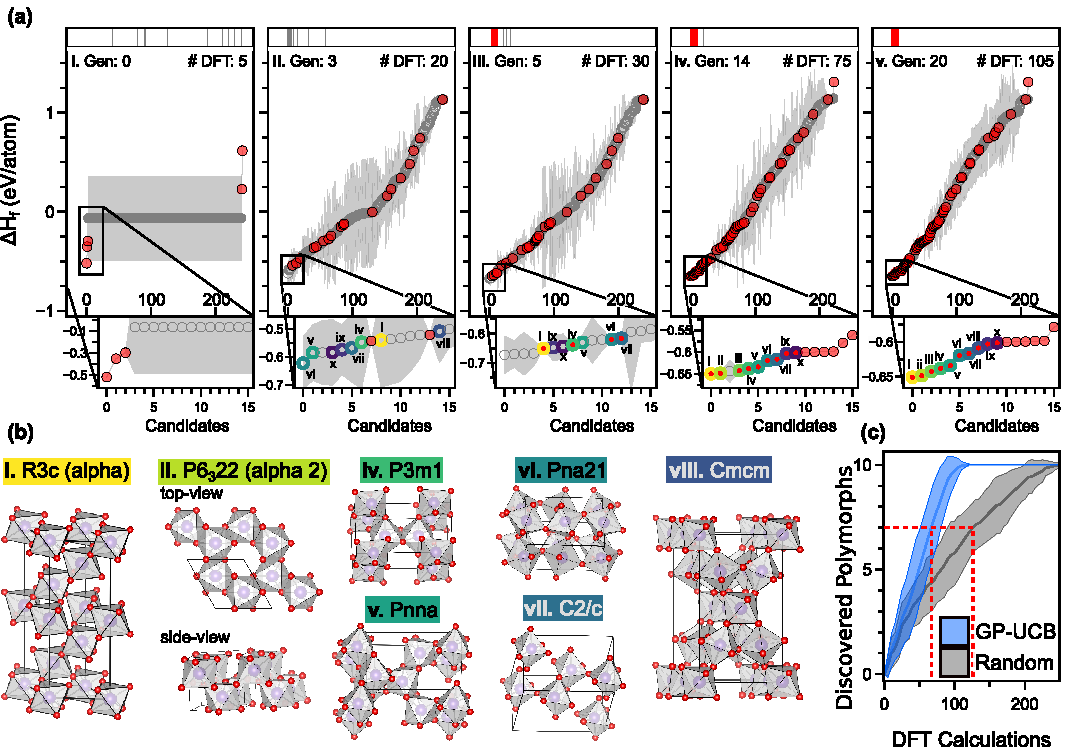
\includegraphics[width=\textwidth,height=\textheight,keepaspectratio]
{02_figures/ml_convergence_plots/test_iro3_al.pdf}
}
\caption{\label{fig:iro3_al}
% (a) %%%%%%%%%%%%%%%%%%%%%%%%%%%%%%%%%%%%%%%%%%%%%%%%%%%%%
%
(a) The state of the AL algorithm at five generations.
%
The enthalpy of formation per atom (\DHf) is plotted, ordered by stability, against all \IrOthree candidates, with the 1 $\sigma$ uncertainty estimate shown for each prediction.
%
The number of DFT training points at each generation is displayed.
%
Hollow grey markers indicate a GP model predicted \DHf while red indicate a DFT-computed quantity.
%
At the top of subplots a.i - a.v, the x-axis positions of the ten most stable polymorphs are tracked at each generation by either red (acquired) or grey (not acquired) vertical lines.
%
Insets of the low energy region for each generation is displayed below each subplot.
%
The top ten most stable systems are colored and labeled (i-vii) to indicate their identity.
% (b) %%%%%%%%%%%%%%%%%%%%%%%%%%%%%%%%%%%%%%%%%%%%%%%%%%%%%
%
(b) Crystal structures of the \num{8} most stable \IrOthree polymorphs (structure iii. not shown).
%
% (c) %%%%%%%%%%%%%%%%%%%%%%%%%%%%%%%%%%%%%%%%%%%%%%%%%%%%%
%
(c) The number of most stable \num{10} polymorphs of \IrOthree discovered vs the number of DFT calculations for the GP-LCB (blue) and random (grey) acquisition methods.
%
The results are averaged over \num{100} independent runs and the 1 $\sigma$ standard deviation between these runs are displayed.
%
Red guidelines show the number of DFT calculations needed to discover \num{7/10} of the most stable polymorphs.
}
\end{figure*}
% __| =====================================================
% =========================================================


% %%%%%%%%%%%%%%%%%%%%%%%%%%%%%%%%%%%%%%%%%%%%%%%%%%%%%%%%%
% | - Parity Plot Discussion
% Discussion on performance of the AL routine
% __|
% %%%%%%%%%%%%%%%%%%%%%%%%%%%%%%%%%%%%%%%%%%%%%%%%%%%%%%%%%
% | - PARAGRAPH BODY
We next evaluate the prediction accuracy of the \IrOtwo and \IrOthree GP regression models utilizing the full DFT optimized data set of 487 \IrOtwo and 249 \IrOthree structures.
%
This dataset corresponds to the final generation of the AL algorithm in which all structures have been acquired.
%
Figure~\ref{fig:parity} plots the GP model predicted \DHf against the DFT-computed values for two special cases.
%
Case 1) shows the predictions on the structural fingerprints prior to DFT-optimization (grey), as is done in the regular operation of the algorithm.
%
Case 2) shows the prediction of the same GP model using the post-DFT optimized fingerprints (blue) with \num{10}-fold cross-validation.
%
It is evident that using the pre-optimization fingerprints results in the GP model being inaccurate in quantitatively predicting the post-relaxation DFT formation energy of the candidate space,
with a seemingly large MAE of \mytilde\num{1.5} eV/atom.
%
The same GP model does comparatively much better at predicting the formation energies of post-DFT optimized structures with an MAE of \mytilde\num{0.2} eV/atom.
% __|
%%%%%%%%%%%%%%%%%%%%%%%%%%%%%%%%%%%%%%%%%%%%%%%%%%%%%%%%%%%



% %%%%%%%%%%%%%%%%%%%%%%%%%%%%%%%%%%%%%%%%%%%%%%%%%%%%%%%%%
% | - Detailed Analysis of Pre vs. Post DFT Predictions
%
% __|
% %%%%%%%%%%%%%%%%%%%%%%%%%%%%%%%%%%%%%%%%%%%%%%%%%%%%%%%%%
% | - PARAGRAPH BODY
%
The apparent discrepancy between the predictive capability on structures fingerprinted before and after relaxation is intriguing in terms of the general utility of AL in DFT datasets,
and has implications on the effectiveness of our approach.
%
Additionally, the drastic decrease in prediction error is not surprising,
since the post-DFT fingerprints directly correspond to the target \DHf values,
and is primarily due to the large degree of structural drift that occurs during DFT relaxation,
the extent of which is not known \latin{a priori}.
%
In fact, we observe that most of the predictions from pre-DFT features over-predict the formation energy (i.e. less stable than their DFT analogous) and lie above the x=y line.
%
This behavior is consistent with what one would expect thermodynamically:
structures that are initialized in high energy configurations will  naturally reconfigure into a more stable local configuration,
resulting in a large discrepancy between the pre-DFT predicted and final formation energies.
%
In practice, the approach still performs notably well by discovering 7 out of the 10 most stable structures with only 35 DFT calculations, because (i) the energy tends to decrease post-DFT relaxation,
meaning favored acquisitions are likely to perform even better,
and (ii) the pre-optimized structures that are similar enough to the most stable final equilibrium structures will not restructure considerably,
meaning that their predicted formation energies will be close enough (and low enough) to be quickly picked up by the acquisition criteria.
%
Additionally, the number of duplicates produced during the AL is also a factor.
%
For example, there are \num{8} duplicates of the \aIrOthree polymorph produced throughout the AL algorithm due to structures relaxing into the same energy basin,
and this over representation of the \aIrOthree phase effectively increases the chance of it being acquired by a factor of eight.
% __|
%%%%%%%%%%%%%%%%%%%%%%%%%%%%%%%%%%%%%%%%%%%%%%%%%%%%%%%%%%%





% %%%%%%%%%%%%%%%%%%%%%%%%%%%%%%%%%%%%%%%%%%%%%%%%%%%%%%%%%
% | - Out Model's Accuracy vs. MP Models
% COMBAK Fix this paragraph and include
% __|
% %%%%%%%%%%%%%%%%%%%%%%%%%%%%%%%%%%%%%%%%%%%%%%%%%%%%%%%%%
% | - PARAGRAPH BODY
% The same GP model does comparatively much better at predicting the formation energies of post-DFT optimized structures with an MAE of \mytilde\num{0.2} eV/atom,
% roughly 120 meV/atom larger than model reported by Ward \latin{et al.}, which was trained on hundreds of thousands of DFT bulk calculations and reached an MAE of 0.8 eV/atom.
% %
% The fact that our models,
% trained on orders of magnitude less data than those of Ward \latin{et al.},
% achieve errors on par with them,
% is due to the fact that we are training and predicting on a space whose properties are very narrowly constrained, while Ward \latin{et al.} is predicting on structures whose elements span the entire periodic table.
% __|
%%%%%%%%%%%%%%%%%%%%%%%%%%%%%%%%%%%%%%%%%%%%%%%%%%%%%%%%%%%


% =========================================================
% FIGURE ==================================================
% | - Figure | IrO2/3 Parity Plot
\begin{figure*}[!htb]
\centering
\makebox[\textwidth][c]{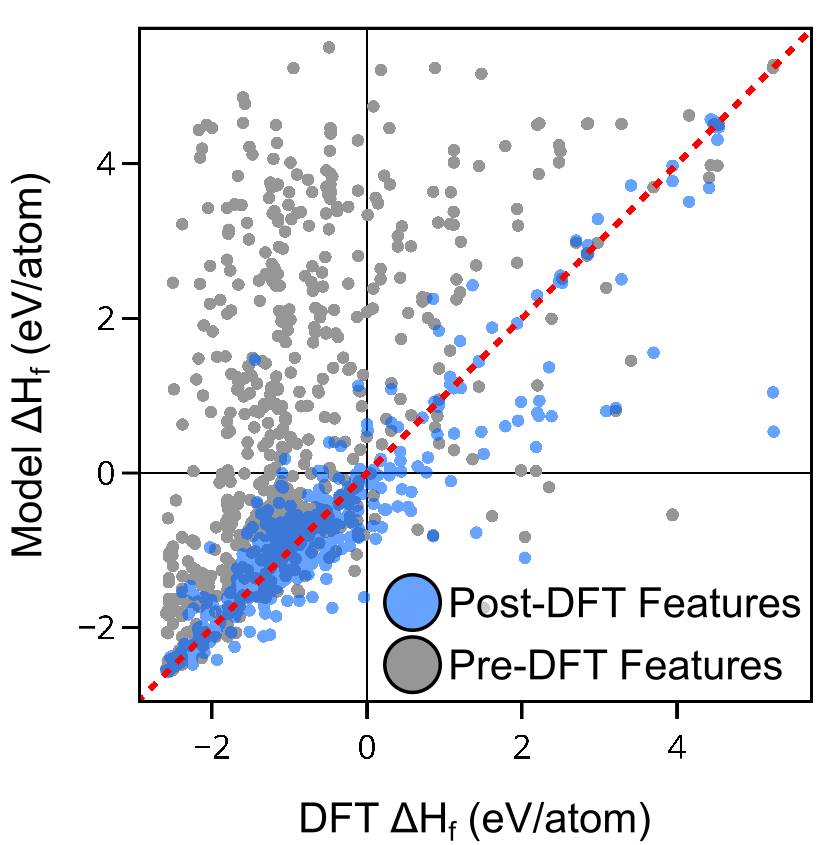
\includegraphics[]
{02_figures/parity_plot.png}
}
\caption{\label{fig:parity}
%
Parity plot of the final ML models for \IrOtwo and \IrOthree predicting on either the pre-optimized (grey) or the post-optimized structures of \IrOtwo and \IrOthree.
}
\end{figure*}
% __|
% =========================================================
